% \newcommand\testfigure{

% \begin{figure}
%   \centering
%   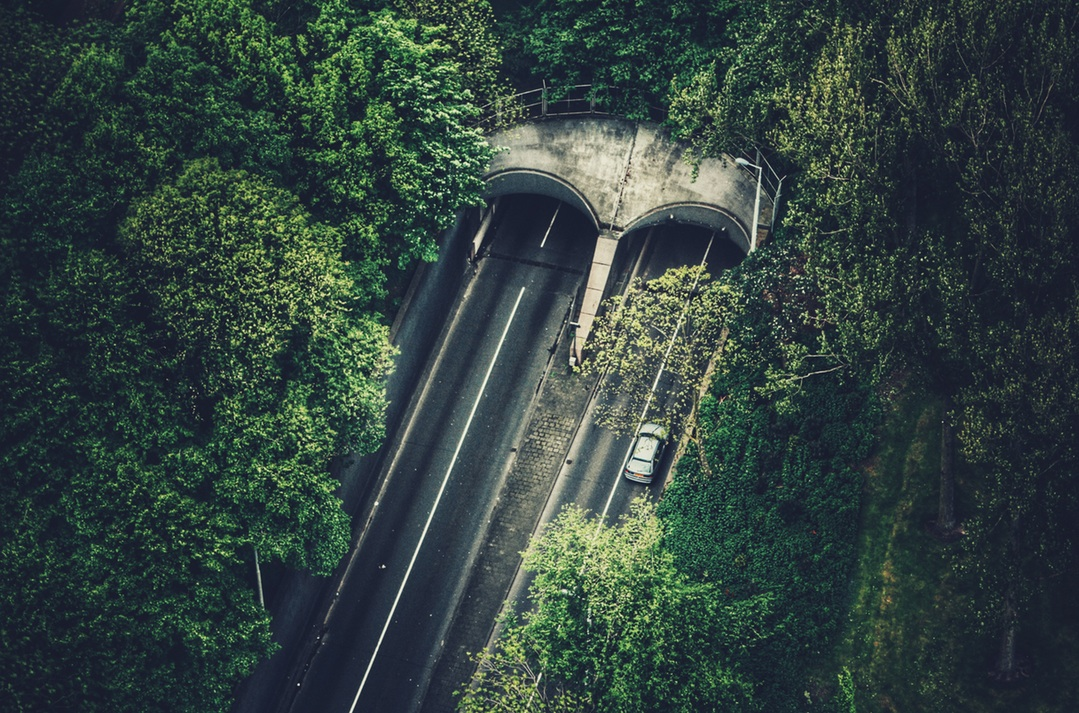
\includegraphics[width=\columnwidth]{img/test}
%   \caption{
%     Please see \S\ref{sec:conclusion}.
%   }
%   \label{fig:protein-validate}
% \end{figure}

% }

\newcommand\guessAError{
  \begin{figure}
    \centering
    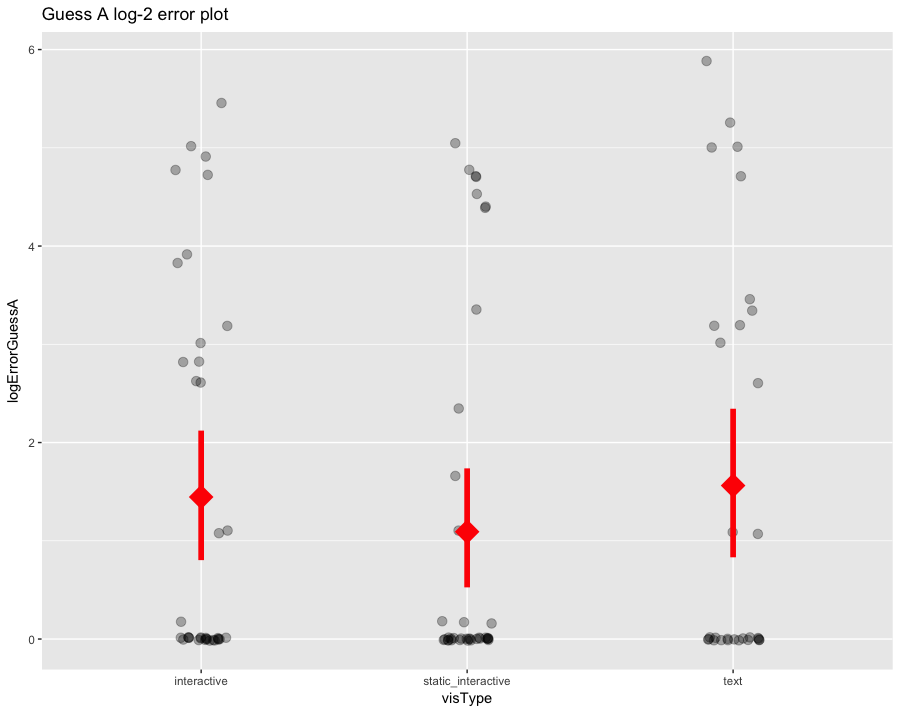
\includegraphics[width=\columnwidth]{img/logError-guessA-104}
    \caption{
      Log error of first lab experiment question.
    }
    \label{fig:guessAErr}

  \end{figure}
}

\newcommand\guessBError{
  \begin{figure}
    \centering
    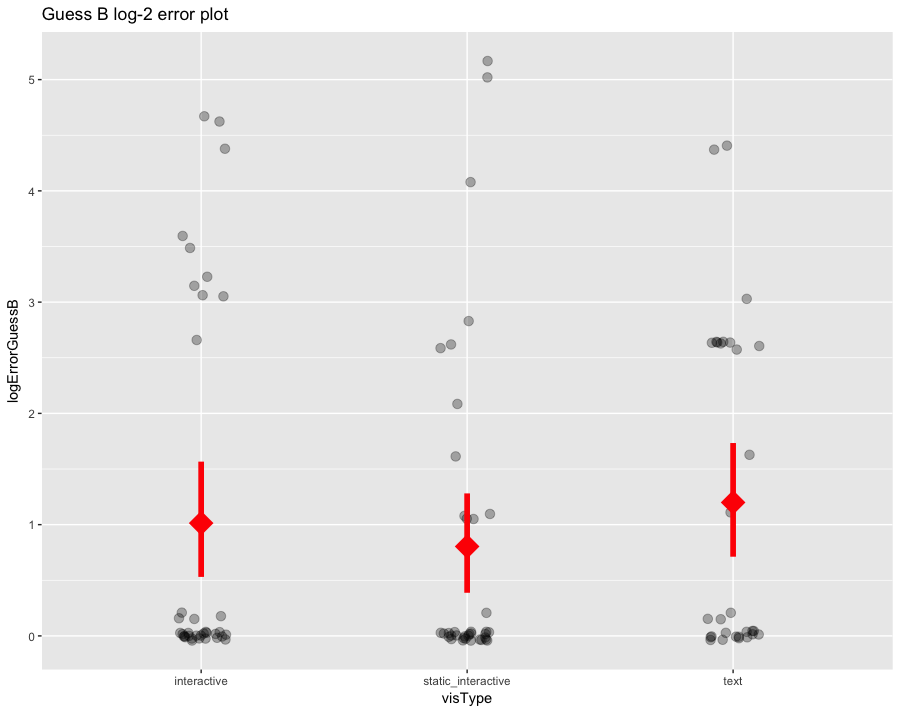
\includegraphics[width=\columnwidth]{img/logError-guessB-104}
    \caption {
      Log error of the second experiment question
    }
    \label{fig:guessBError}
  \end{figure}
}

\newcommand\accuracyPlot{
  \begin{figure}
    \centering
    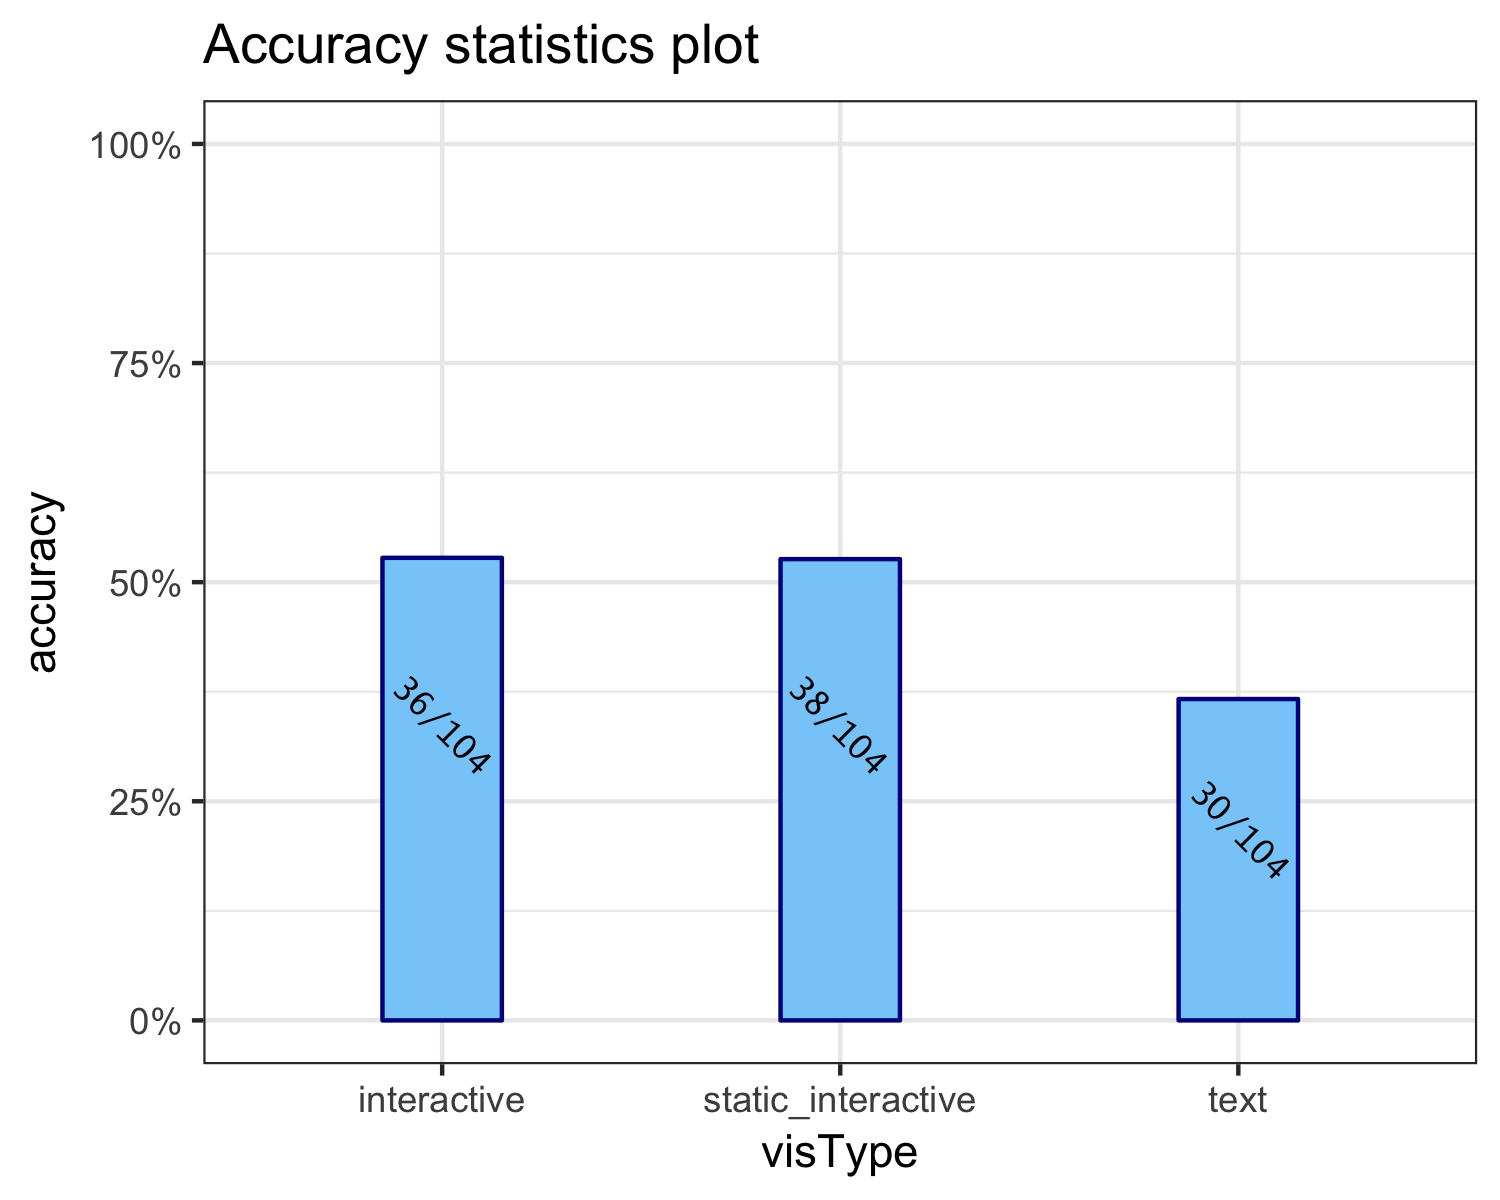
\includegraphics[width=\columnwidth]{img/Accuracy-edit}
    \caption {
      Overall accuracy by visualization type
    }
    \label{fig:accuracyPlot}
  \end{figure}
}

\newcommand\educationAccuracy{
  \begin{figure}
    \centering
    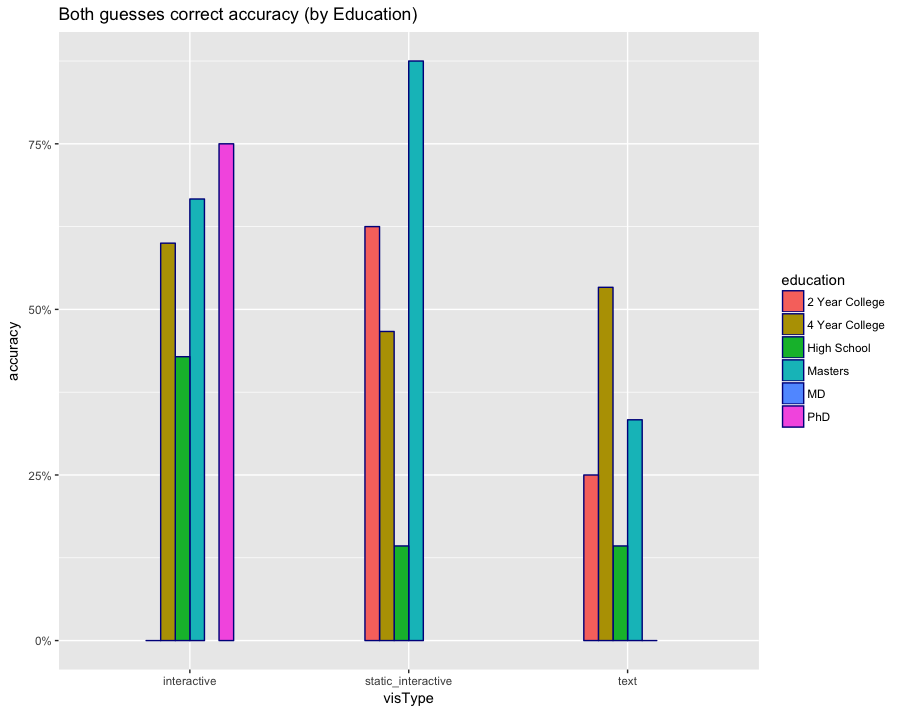
\includegraphics[width=\columnwidth]{img/bothGuessesCorrect-accuracy-byEducation-104}
    \caption {
      Overall accuracy by participants' education
    }
    \label{fig:educationAccuracy}
  \end{figure}
}

\newcommand\experienceAccuracy{
  \begin{figure}
    \centering
    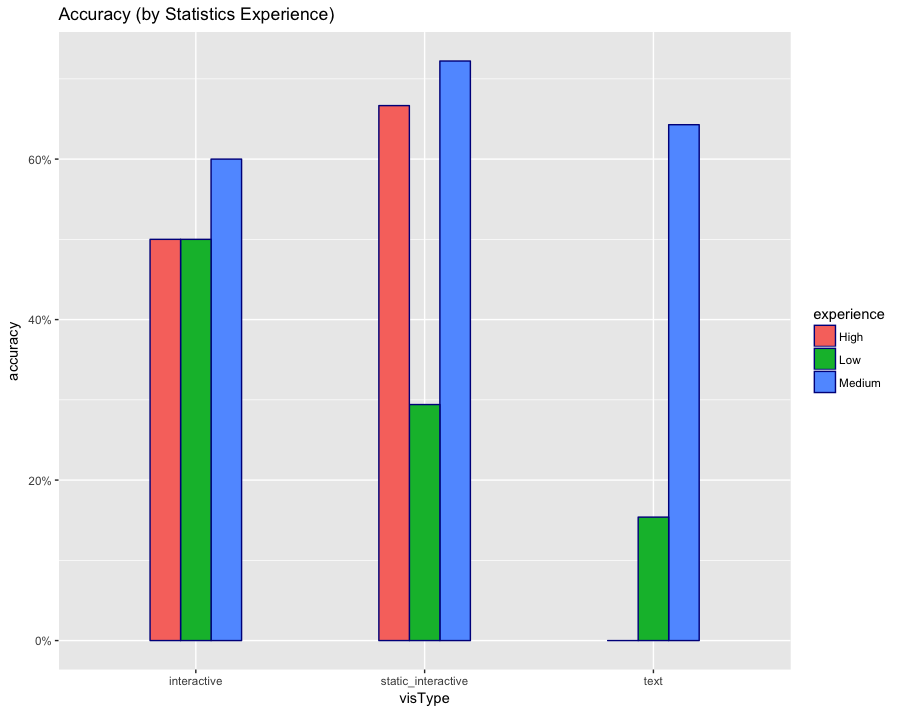
\includegraphics[width=\columnwidth]{img/bothGuessesCorrect-accuracy-byStatExp-104}
    \caption {
      Overall accuracy by participants' statistical experience
    }
    \label{fig:experienceAccuracy}
  \end{figure}
}

\newcommand\interactiveVis{
  \begin{figure}
    \centering
    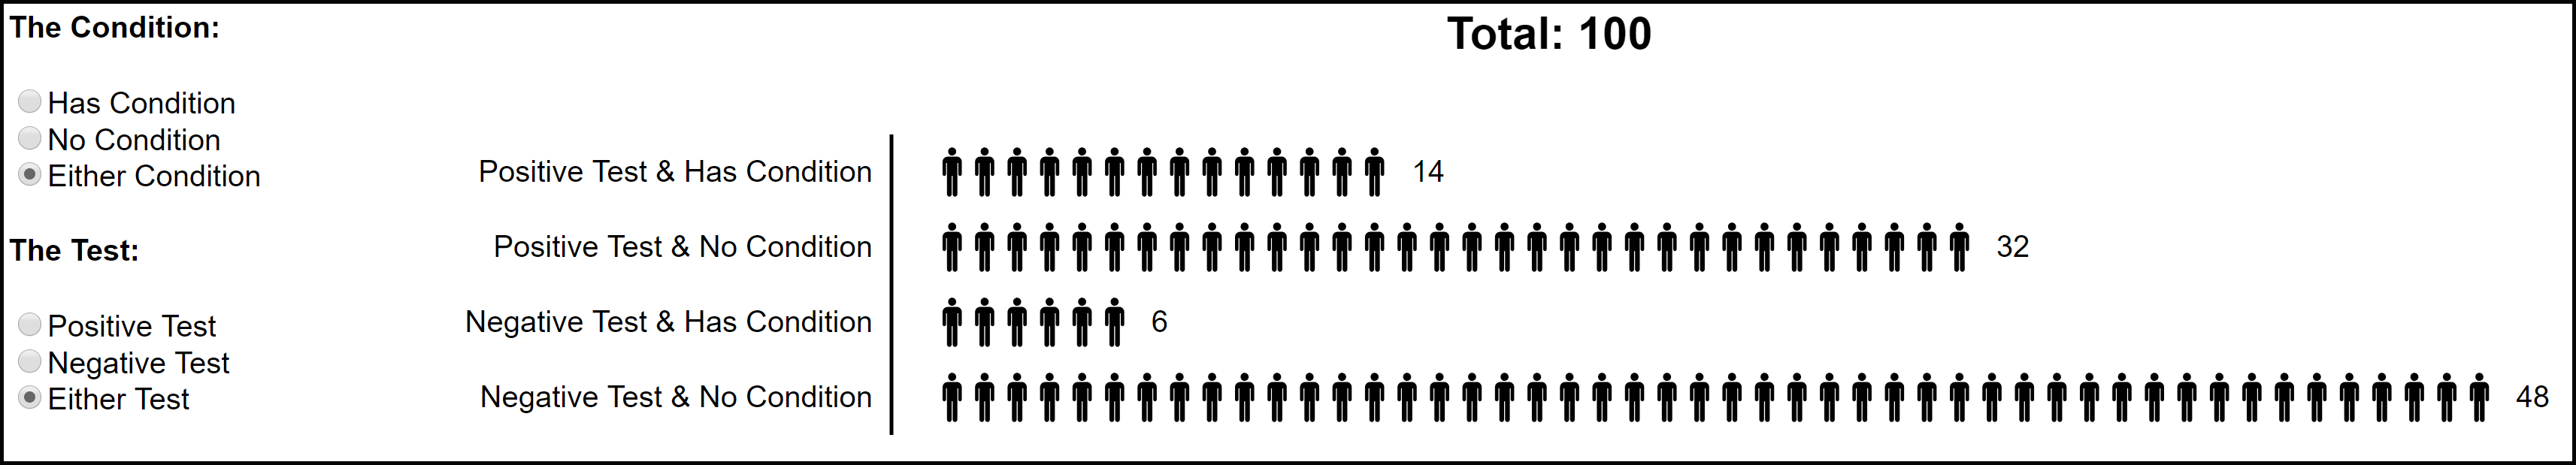
\includegraphics[width=\columnwidth]{img/teaser-EDIT.png}
    \caption{Interactive Visualization for Bayesian Statistics}
    \label{fig:interactive}
  \end{figure}
}

\newcommand\interactiveVisToggle{
  \begin{figure}
    \centering
    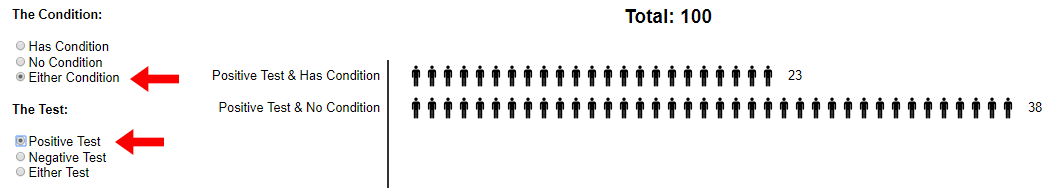
\includegraphics[width=\columnwidth]{img/interactive-toggle-EDIT.png}
    \caption{Interactive Visualization for Bayesian Statistics wit Condition Toggled On}
    \label{fig:interactive-toggle}
  \end{figure}
}

\newcommand\staticVis{
  \begin{figure}
    \centering
    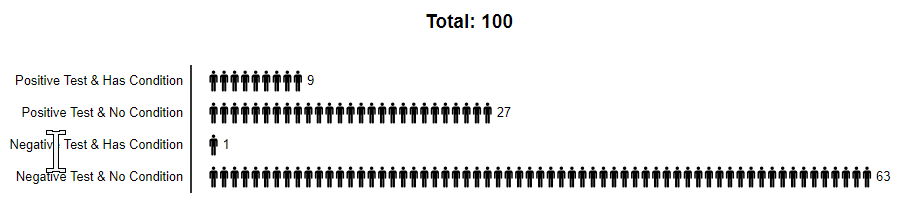
\includegraphics[width=\columnwidth]{img/static}
    \caption{Static Visualization for Bayesian Statistics}
    \label{fig:static}
  \end{figure}
}